Consider a \textit{two}-dimensional, ideal Bose fluid.

\paragraph{a) What is the expression for the mean particle number for a 2D system?
    \textit{(1 point)}
} \ \\
\\
Recall that the particle number $N$ for spin-0 bosons (degeneracy g = 1) 
for a 3D system is given by
\begin{align}
	N = \sum_{\vec{k}} n_{\vec{k}}
	= \frac{V}{h^3} \int \dd \vec{p} \, \frac{1}{e^{\beta (\epsilon(p) - \mu)}-1} \,,
\end{align}
where we encounter the sum over all modes and the Bose distribution. 
The corresponding expression for a 2D system is given by
\begin{align}
	N = \frac{A}{h^2} \int \dd \vec{p} \, \frac{1}{e^{\beta (\epsilon(p) - \mu)}-1}
	= \frac{2\pi A}{h^2} \int_0^{\infty} \dd p \, \frac{p}{e^{\beta (\epsilon(p) - \mu)}-1} \,.
\end{align}

\paragraph{b) First consider particles with energy $\epsilon(p)=\frac{p^2}{2m}$.
	Evaluate the mean particle number and investigate whether there is a Bose-Einstein 
	condensation (BEC) at finite temperature.
    \textit{(2.5 points)}
} \ \\
\\
With the formula from above, we get $\dd p = m \dd\epsilon / p$ and
\begin{align}
	N &= \frac{2\pi A}{h^2} \int_0^{\infty} \dd p \, \frac{p}{e^{\beta (\epsilon(p) - \mu)}-1}
	= \frac{2\pi m A}{h^2} \int_0^{\infty} \dd\epsilon \, \frac{1}{e^{\beta (\epsilon - \mu)}-1} \notag \\
	&= \frac{2\pi m A}{h^2} \sum_{l=1}^{\infty} e^{\beta\mu l} \int_0^{\infty} \dd\epsilon \, e^{- \beta\epsilon l}
	= \frac{2\pi m A}{\beta h^2} \sum_{l=1}^{\infty} \frac{z^l}{l} \notag \\
	&= \frac{A}{\lambda^2} \, g_1(z) \,,
\end{align}
where we introduced the fugacity $z=e^{\beta\mu}$, the thermal wavelength $\lambda=\frac{h}{\sqrt{2\pi m k_B T}}$ 
and the generalized Riemann Zeta function $g_{\nu}(z)=\sum_{l=1}^{\infty}\frac{z^l}{l^{\nu}}$. \\
\\
Plot $g_1(z) = - \ln(1-z)$ from $z=0$ to $z=1$: \\

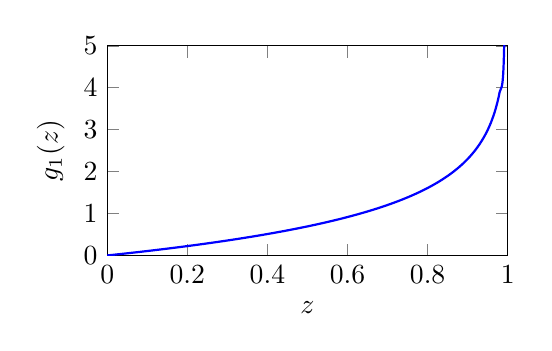
\begin{tikzpicture}
\begin{axis}[
	xmin = 0, xmax = 1,
	ymin = 0, ymax = 5.0,
	xtick distance = 0.2,
	ytick distance = 1.0,
	width = 0.55\textwidth,
	height = 0.35\textwidth,
	xlabel = {$z$},
	ylabel = {$g_1(z)$},]

% Plot a function
\addplot[
	domain = 0:1,
	samples = 100,
	smooth,
	thick,
	blue,
] {-ln(1-x)};
\end{axis}
\end{tikzpicture}
\\ \\
See that it diverges for $z \longrightarrow 1$. Thus, no BEC!


\paragraph{c) Now consider massless bosons with energy $\epsilon(p)=cp$.
	Again evaluate the mean particle number and investigate whether there is a 
	BEC at finite temperature.
    \textit{(2.5 points)}
} \ \\
\\
With the formula from above, we get $\dd p = \dd\epsilon / c$ and
\begin{align}
	N &= \frac{2\pi A}{h^2} \int_0^{\infty} \dd p \, \frac{p}{e^{\beta (\epsilon(p) - \mu)}-1}
	= \frac{2\pi A}{c^2 h^2} \int_0^{\infty} \dd\epsilon \, \frac{\epsilon}{e^{\beta (\epsilon - \mu)}-1} \notag \\
	&= \frac{2\pi A}{c^2 h^2} \sum_{l=1}^{\infty} e^{\beta\mu l} \int_0^{\infty} \dd\epsilon \, \epsilon \, e^{- \beta\epsilon l}
	= \frac{2\pi A}{\beta^2 c^2 h^2} \sum_{l=1}^{\infty} \frac{z^l}{l^2} \notag \\
	&= \frac{2\pi A}{\beta^2 c^2 h^2} \, g_2(z) \,.
\end{align}
Plot $g_2(z) = \text{Li}_2(z)$ from $z=0$ to $z=1$: \\

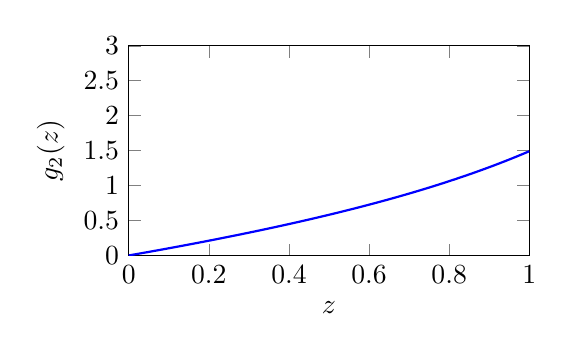
\begin{tikzpicture}
\begin{axis}[
	xmin = 0, xmax = 1,
	ymin = 0, ymax = 3.0,
	xtick distance = 0.2,
	ytick distance = 0.5,
	width = 0.55\textwidth,
	height = 0.35\textwidth,
	xlabel = {$z$},
	ylabel = {$g_2(z)$},]

% Plot a function
\addplot[
	domain = 0:1,
	samples = 100,
	smooth,
	thick,
	blue,
] {x+x*x/4+x*x*x/9+x*x*x*x/16+x*x*x*x*x/25+x*x*x*x*x*x/36};
\end{axis}
\end{tikzpicture}
\\ \\
See that it converges for $z \longrightarrow 1$. Thus, BEC!

\paragraph{d) In case you find a BEC, give the respective expression for the critical temperature.
    \textit{(1 point)}
} \ \\
\\
We have found a BEC for the case of massless particles. \\
When the system reaches the critical temperature, the chemical potential is zero ($\mu=0$). \\
Thus, by defining the particle density $\rho = N/A$, we get
\begin{align}
	\rho = \frac{2\pi}{\beta^2 c^2 h^2} \, g_2(1) \quad \longleftrightarrow \quad
	T_c = \frac{hc}{k_B} \sqrt{\frac{\rho}{2\pi g_2(1)}} = \frac{hc}{k_B} \sqrt{\frac{3\rho}{\pi^3}} \,.
\end{align}